\chapter{导出代数几何}\label{ch:14}

\begin{keytakeaways}
本章解释为什么局部算子比交换代数“多一层”：一个 $n$ 维拓扑场论中，局部算子空间 $A=\cZ(S^{n-1})$ 带有 $\mathbb{E}_n$-代数结构（小 $n$ 圆盘算子代数），而 Dunn–Lurie 可加性 $\mathbb{E}_k+\mathbb{E}_\ell=\mathbb{E}_{k+\ell}$ 解释了它的来源。取上同调后 $\mathbb{E}_n$ 退化为 $\PP_n$-代数：$n=1$ 是普通 Poisson 代数，$n=2$ 是 Gerstenhaber 代数，$n\ge3$ 是（分次）Poisson 代数。于是非交换的 $\mathbb{E}_n$-代数应看成 $\PP_n$-代数的量子化，其“经典极限”是移位辛（shifted symplectic）簇；B-模型的真空模空间正是 $T^*[1]X$，它上面的形变量子化给出可观测量的代数 $\mathrm{HH}^*$，而几何量子化给出态范畴 $\QC(X)$。最后讨论切向结构（定向 vs 标架）如何迫使我们在 $\mathrm{HH}_*$ 与 $\mathrm{HH}^*$ 之间选一个等同，即选一个体积形式。
\end{keytakeaways}

\section{拓扑场论与 $\mathbb{E}_n$-代数}\label{sec:14-1}

\begin{sectionkey}
本节从拓扑扭转出发，说明 TFT 中“局部算子”为什么天然带有 $\mathbb{E}_n$-代数结构：它来自把 $k$ 个小圆盘嵌入大圆盘的构型空间的作用。核心是把“结合积”升级为“构型空间参数化的多重复积”，这也是 $\mathbb{E}_n$ 定义的几何来源。
\end{sectionkey}

对物理学家来说，拓扑场论大致有两个来源。第一个来源是那些我们可以直接写下来、明显是拓扑的理论，例如有限群例子和 Chern–Simons 理论。但大多数有趣的拓扑理论不是这样产生的。第二个来源是由拓扑扭转产生的理论。

\term{拓扑扭转}{topological twisting}的想法如下。从一个“诚实的”（欧氏的）量子场论出发。它是定义在 Riemann 流形范畴上的某种函子。然后某些特殊的量子场论具有超对称（SUSY）。这意味着我们有某个有趣的超李代数的作用。有特定的算子 $Q$，称为 BRST 算子，它们是我们的态空间上的奇、次数 1 的自同态。于是我们有一个满足 $Q^2=0$ 的算子，因此可以过渡到上同调。

大多数 QFT 不是 SUSY 的，大多数 SUSY 理论也不是拓扑的。但人们常常发现理论具有这样的结构：所谓的应力张量 $T$ 是 $Q$-恰当的。注意这是一种\emph{结构}而不是\emph{性质}。应力张量是（物理中）描述对几何/度规变化的响应的对象。所以如果这种对几何变化的依赖是 $Q$-恰当的，那么在上同调层面，理论就不依赖于几何。实际上，应力张量控制我们的场论 $Z$ 在 Riemann 流形模空间上的变化。例如，从 $S^1\sqcup S^1$ 到 $S^1$ 的 Riemann 配边构成整个空间。于是 $Z$ 把它送到一族映射 $Z(S^2)^{\otimes2}\to Z(S^1)$。它是 $Q$-恰当的这一事实意味着，在上同调层面，这种对几何的依赖是局部常值的。

% [Tutor Note: 上一段末尾的 $Z(S^{2})^{\otimes 2}\to Z(S^{1})$ 疑为原书笔误：$\Sigma$
% 是从 $S^{1}\sqcup S^{1}$ 到 $S^{1}$ 的配边，故 $Z(\Sigma)$ 应是
% $\Hom\bigl(Z(S^{1})^{\otimes 2},Z(S^{1})\bigr)$ 中的族，紧接的 (14.1)(14.2) 也正写作
% $Z(S^{1})^{\otimes 2}$；译文照印本保留 $S^{2}$，不改动数学。
% [译者按（无外部依据）：由同段 (14.1) 的内部一致性判定，未找到外部依据。]]
当我们有一个 TFT $Z$ 时，如果 $\Sigma$ 是从 $S^1\sqcup S^1$ 到 $S^1$ 的配边，即带三个穿孔的曲面，那么我们预期 $Z(\Sigma)$ 是所有这类配边的模空间上的局部常值函数，取值于
\begin{equation}\tag{14.1}
\Hom\left(Z(S^1)^{\otimes2},Z(S^1)\right).
\end{equation}
在链的层面，我们可以把它改写为
\begin{equation}\tag{14.2}
Z\in\Hom\left(Z(S^1)^{\otimes2},Z(S^1)\right)\otimes C^*(M).
\end{equation}
或者等价地，它定义了一个映射
\begin{equation}\tag{14.3}
C_*(M)\otimes Z(M_{in})\to Z(M_{out}).
\end{equation}
% [Tutor Note: (14.1)--(14.3) 是同一件事的三种说法：$Z(\Sigma)$ 在配边模空间上局部
% 常值，即 $Z$ 给出该模空间上的局部常值链复形（局部系统），故 (14.2) 把它写成
% $\Hom(\cdots)\otimes C^{*}(M)$；再用张量–$\Hom$ 伴随把 $C^{*}(M)$ 搬到另一侧，
% 就是 (14.3) 的 $C_{*}(M)\otimes Z(M_{\mathrm{in}})\to Z(M_{\mathrm{out}})$。原书
% (14.2) 用上标 $C^{*}$、(14.3) 用下标 $C_{*}$，互为对偶（$C^{*}\cong(C_{*})^{\vee}$），经张量–$\Hom$ 伴随等同；译文照原文未统一写法。
% [译者按（无外部依据）：由 (14.1)--(14.4) 的内部一致性判定。]]

另一种写法如下。设 $|M|$ 为 Riemann 配边的模空间。这是空间 $M$ 底层的同伦型/anima/$\infty$-群胚。那么这等同于一个映射
\begin{equation}\tag{14.4}
|M|\to\Hom(Z(M_{in}),Z(M_{out})).
\end{equation}
在范畴层面我们得更小心“局部常值”是什么意思，即我们需要区分 de Rham 与 Betti 设定。我们或许会看从 $M$ 的 de Rham 空间到“运算”的映射，这可以称为 de Rham 场论。Betti 版本则考虑从 $|M|$ 到“运算”的映射。在函数/向量空间的层面这没有区别，但局部常值层有两个版本：一个平坦联络并不会自动给你平行移动。

\subsection{局部算子上的 $\mathbb{E}_n$-代数结构}\label{sec:14-1-1}

我们假定处在这个局部常值/Betti 的情形。我们想关注局部算子上得到的结构。回忆我们有过这样的想法：局部算子空间
\begin{equation*}
A=\cZ(S^{n-1})
\end{equation*}
作用在 $\cZ(M^{n-1})$ 上，对任何 $(n-1)$-流形 $M^{n-1}$。现在我们将在导出的设定中重新审视这一点。当我们想复合局部算子时，我们画的图如下：
\diagram[0.14\textwidth]{p243_d1.png}
它给出乘法：
\begin{equation}\tag{14.5}
A^{\otimes2}\to A.
\end{equation}
对 $n>1$，球可以互相移动，于是我们得到交换的乘法（在非导出层面）。更好的说法是
\begin{equation}\tag{14.6}
H_0\bigl(\mathrm{Conf}_2(D^n)\bigr)=\Z,
\end{equation}
即 $D^n$ 中两点的构型空间是连通的。一般地，场论给我们一个映射
\begin{equation}\tag{14.7}
\mathrm{Conf}_k(D^n)\to\Hom\left(A^{\otimes k},A\right).
\end{equation}
当我们过渡到导出设定，这就是所谓的 $\mathbb{E}_n$-代数的定义。即 $A$ 是小 $n$ 圆盘\term{操作子}{operad}上的代数。这告诉我们有一个映射
\begin{equation}\tag{14.8}
C_*\bigl(\mathrm{Conf}_k(D^n)\bigr)\to\Hom\left(A^{\otimes k},A\right).
\end{equation}
拓扑上，我们可以简单地说有一个映射
\begin{equation}\tag{14.9}
\left|\mathrm{Conf}_k(D^n)\right|\to\Hom\left(A^{\otimes k},A\right).
\end{equation}
于是就给出了任何对称幺半高阶范畴中 $\mathbb{E}_n$-代数的概念。
% [Tutor Note: (14.5)--(14.9) 的关键是“构型空间参数化运算”：$n=1$ 时 $\mathrm{Conf}_k(D^1)$ 不连通（有 $k!$ 个分量），给出结合的乘法和置换；$n>1$ 时连通，给出交换乘法。所谓“导出”就是把 $\mathrm{Conf}_k(D^n)$ 换成它的链复形/同伦型，从而把“只在同伦意义下交换”精化为 $\mathbb{E}_n$ 结构。切勿把 (14.7) 读成“每个构型给一个映射”，它在导出层面是一个 $\mathrm{Conf}_k$ 上的局部系统。]
% [Tutor Note: 上文“操作子”是 operad 的译名（May 意义下的“小 $n$ 圆盘”operad：
% 每个 $k$ 给构型空间 $\mathrm{Conf}_k(D^n)$，用其链复形记录 $k$ 元运算及其替换），
% 与泛函分析里的 operator algebra 无关。第 11、15 章在同样语境下直接写英文
% operad，本仓库资料卡作“操作子”，三种写法尚未统一，读时按 operad 理解即可。
% [来源：本仓库资料卡 functoriality/concept/operad]]

\begin{srcrem}{99}
我们可以在任何对称幺半高阶范畴中定义 $\mathbb{E}_n$-代数的概念，但有时该范畴被假定为链复形范畴，这时人们就径称 $\mathbb{E}_n$-代数。
\end{srcrem}

\begin{srcex}{94}
在（普通/离散/非导出）$\Vect$ 中的 $\mathbb{E}_n$-代数，对 $n=1$ 就是结合代数，对 $n>1$ 就是交换代数。
\end{srcex}

\begin{srcex}{95}
在（普通/离散/非导出）$\mathrm{Cat}$ 中的 $\mathbb{E}_n$-代数：$n=1$ 是幺半范畴，$n=2$ 是编织幺半范畴，$n>2$ 是对称幺半范畴。
\end{srcex}

\subsection{$\mathbb{E}_n$-代数的来源}\label{sec:14-1-2}

$\mathbb{E}_n$-代数的“原初”例子如下。设 $X$ 是带基点的拓扑空间。考虑 $X$ 中的 $n$ 重基点环路空间 $\Omega^nX$。我们应该把它想成
\begin{equation}\tag{14.10}
\mathrm{Map}\left((\R^n,\R^n\setminus D^n),(X,*)\right)=\mathrm{Map}\left(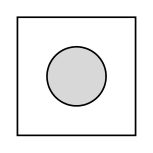
\includegraphics[width=0.045\textwidth]{p244_d1.png},(X,*)\right).
\end{equation}
即从 $\R^n$ 到 $X$ 的映射空间，使得 $D^n\subset\R^n$ 的补集映到基点。通过把多个圆盘放进一个更大的圆盘，我们得到复合映射。于是我们得到一个映射
\begin{equation}\tag{14.11}
\left|\mathrm{Conf}_kD^n\right|\times(\Omega^nX)^k\to\Omega^nX.
\end{equation}
即 $\Omega^nX$ 是空间范畴中的 $\mathbb{E}_n$-代数。这是“对 $n>1$，$\pi_n(X)$ 交换”这一事实的花哨版本：
\begin{equation}\tag{14.12}
\pi_0(\Omega^nX)=\pi_n(X).
\end{equation}

\begin{srcthm}{14（识别定理）}
若 $Y$ 是足够连通的空间，则把 $Y$ 与某个 $n$ 重环路空间等同起来，$Y\overset{\sim}{\longrightarrow}\Omega^nX$，对应于 $Y$ 上的 $\mathbb{E}_n$-结构。
\end{srcthm}

\subsection{可加性}\label{sec:14-1-3}

关于 $\mathbb{E}_n$-代数最重要的想法是它们满足某个版本的可加性。我们将使用的版本称为 Dunn–Lurie 可加性，它说
\begin{equation}\tag{14.13}
\mathbb{E}_k+\mathbb{E}_\ell=\mathbb{E}_{k+\ell}.
\end{equation}
我们先前见过它的一个基本版本：如果我们有两个相容的结合运算，那么它们被迫相等且交换。所以这在更大的一般性下成立：$\mathbb{E}_\ell$-代数中的 $\mathbb{E}_k$-代数是一个 $\mathbb{E}_{k+\ell}$-代数。理解这一点的一种方式是：它告诉我们 $\mathbb{E}_n$ 是什么意思——它是装备了 $n$ 个相容结合积的对象。

\subsection{范畴表现}\label{sec:14-1-4}

$\mathbb{E}_n$-代数可以看成 $n$-截断的 $n$-范畴。结果这实际上是一个等价。

$\mathbb{E}_1$-代数是结合代数的导出版本。即它是幺半群，也就是带单个对象 $(\cC,*)$ 的范畴。对 $(\cC,*)$ 我们可以附上代数 $\End(*)$。反方向上，给定代数 $A$，我们可以附上带单个对象 $*$、其自同态由 $\End(*)=A$ 给出的范畴 $BA$。这就是 $\mathbb{E}_1$-代数与带单个对象的范畴之间的对应：
\begin{align}
\End(*)&\leftarrow(\cC,*) \tag{14.14}\\
A&\mapsto BA. \tag{14.15}
\end{align}
类似地，我们可以考虑带一个对象 $*$ 和一个 1-态射 $1_*$ 的 2-范畴。那么我们可以把它送到结合代数 $A=\End(1_*)$。但这个单态射 $1_*$ 是 1-态射复合的单位。$1_*$ 与自身的复合给出 $A$ 上新的结合结构，即由可加性，$A$ 事实上是 $\mathbb{E}_2$-代数。于是这个 2-截断 2-范畴给了我们一个 $\mathbb{E}_2$-代数。

我们也可以做介于两者之间的事情。给定 1-截断的 2-范畴 $(\cC,*)$（即带单个对象的 2-范畴），我们可以考虑 $A=\End(*)$，它是幺半（$\mathbb{E}_1$）范畴。结果 1-截断 2-范畴等价于 $\mathbb{E}_1$-范畴。

想法是：如果我们有一个 $n$-范畴，并且它是 $n$-截断的（即一路下去只有一个 $n$-态射），那么我们就会发现
\begin{equation}\tag{14.16}
A=\End\left(1_{1\cdots1}\right)
\end{equation}
有 $n$ 个相容乘法。所以 $\mathbb{E}_n$ 中的 $n$ 与 $n$-范畴中的 $n$ 是同一个 $n$。这总结在高阶范畴的周期表中，即表 14.1。
% [Tutor Note: (14.16) 中的 $1_{1\cdots1}$ 是“一路复合到底”的单个 $n$-态射的记号，原书用嵌套下标表示（$1_{1_{\cdot_{\cdot}}}$）；这里按行文线性化为 $1_{1\cdots1}$，含义不变：这个自同态代数带有 $n$ 个相互相容的乘法。]

\begin{table}[htbp]
\centering
\caption{高阶范畴的周期表。BTC 代表编织张量范畴。（原文 p.~244，Table 14.1）}
\label{tab:14-1}
\small
\begin{tabular}{c|ccc}
\toprule
\multicolumn{1}{c}{} & \multicolumn{3}{c}{cat\#}\\
\cmidrule(lr){2-4}
truncated\# & 1 & 2 & 3\\
\midrule
1 & $\mathbb{E}_1$-algebra & $\mathbb{E}_1$-category & $\mathbb{E}_1$ 2-category\\
2 & & $\mathbb{E}_2$-algebra & $\mathbb{E}_2$-category (BTC)\\
3 & & & $\mathbb{E}_3$-algebra\\
\bottomrule
\end{tabular}
\end{table}

与其看这些带单个对象的小截断范畴，我们可以谈论由单个对象\emph{生成}的范畴。我们希望有结合（$\mathbb{E}_1$）代数与带点（$\mathbb{E}_0$）范畴之间的字典。对 $(\cC,*)$ 为 $\mathbb{E}_0$-范畴，我们可以附上结合代数 $\End(*)$。反方向上，给定结合代数 $A$，我们可以把它送到范畴 $A\text{-}\mathbf{mod}$，并带一个被指定的对象 $A\in A\text{-}\mathbf{mod}$。函子 $\End(*_{(-)})$ 与 $(-)\text{-}\mathbf{mod}$ 互为伴随。这是把上述字典换一种写法（$BA$ 可以从 $A\text{-}\mathbf{mod}$ 恢复），但现在范畴有余极限之类的东西，于是表示论中感兴趣的范畴就纳入这个框架。

\begin{srcex}{96}
设 $\cC$ 是幺半（$\mathbb{E}_1$）范畴。那么我们有一个结合代数
\begin{equation}\tag{14.17}
\End(1_{\cC})=A.
\end{equation}
但这实际上是 $\mathbb{E}_2$-代数，因为 $1_{\cC}$ 是单位。并且我们有嵌入
\begin{equation}\tag{14.18}
A\text{-}\mathbf{mod}\hookrightarrow\cC.
\end{equation}
如果 $A$ 是 $\mathbb{E}_2$-代数，那么 $A\text{-}\mathbf{mod}$ 事实上是幺半的。即取 $-\text{-}\mathbf{mod}$ 会把你降一个 $\mathbb{E}_n$ 层级。
\end{srcex}

\begin{srcex}{97}
如果 $A$ 是 $\mathbb{E}_n$-代数，那么 $A\text{-}\mathbf{mod}$ 是 $\mathbb{E}_{n-1}$-范畴。于是我们可以取这个范畴并寻找它的模：$A\text{-}\mathbf{mod}\text{-}\mathbf{mod}$，它是 $\mathbb{E}_{n-2}$-2-范畴。我们可以把这个过程继续 $n$ 次，得到一个 $n$-范畴：
\begin{equation}\tag{14.19}
A\text{-}\mathbf{mod}\cdots\text{-}\mathbf{mod}=A\text{-}\mathbf{mod}^n.
\end{equation}
\end{srcex}

\begin{srcrem}{100}
这都是说 $n$-范畴基本上只是 $\mathbb{E}_n$-代数的更花哨/更一般的版本。就像范畴是结合代数的花哨版本，只不过我们只有这种部分定义的乘法。
\end{srcrem}
% [Tutor Note: 表 14.1 在原文中是一张 4×4 的排版表（p.~244），图文件 \texttt{table14-1.png} 的裁剪把表后正文一并包含进来、不宜直接插图，故按本书规范（guide §3.3：能可靠重排则优先重排）用 booktabs 重排；内容与原文逐格一致。]
% 若确需用图像版，可改为：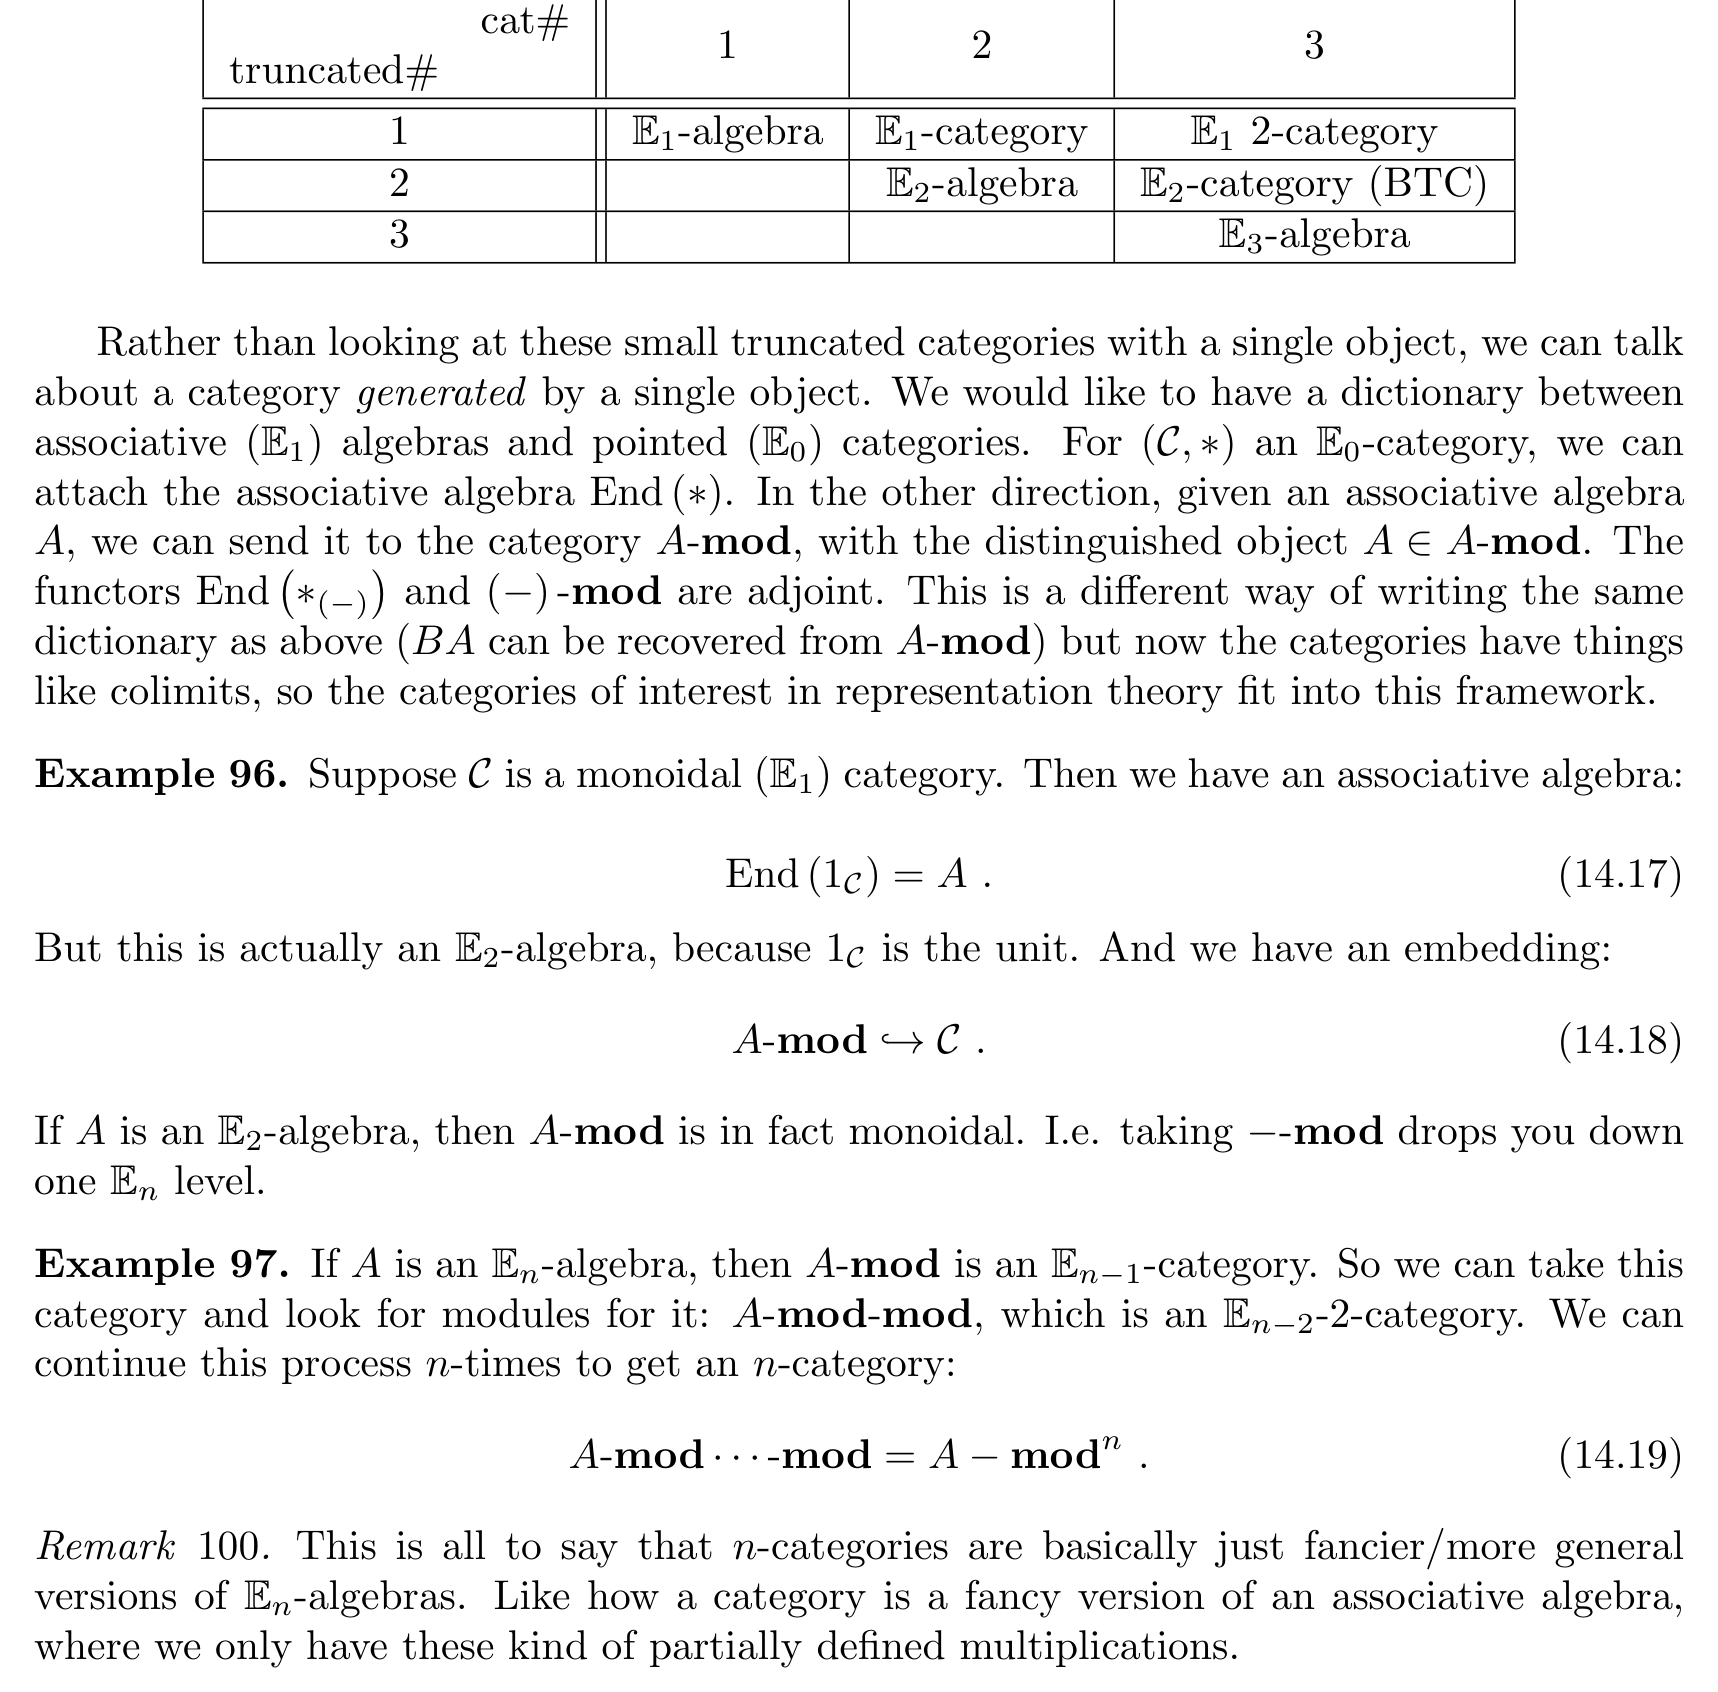
\includegraphics[trim=0 1332 0 0,clip,width=0.85\textwidth]{table14-1.png}（裁去表后正文）。

\section{Hochschild 上同调}\label{sec:14-2}

\begin{sectionkey}
本节说明结合代数 $A$ 的中心/Hochschild 上同调 $\mathrm{HH}^*(A)=\End_{A\text{-}\mathbf{mod}\text{-}A}(A)$ 天然是 $\mathbb{E}_2$-代数（Deligne 猜想，由 Dunn–Lurie 可加性推出），并在上同调层面退化为 Gerstenhaber 代数：一个次数 0 的交换乘法加上一个次数 $-1$ 的 Poisson 括号。HKR 定理把它具体化为外代数 $\wedge^\bullet T_M$ 上的 Schouten–Nijenhuis 括号。
\end{sectionkey}

对 $A$ 为结合代数，我们附上它的中心/Hochschild 上同调
\begin{equation}\tag{14.20}
Z(A)=\mathrm{HH}^*(A)=\End_{A\text{-}\mathbf{mod}\text{-}A}(A).
\end{equation}
Gerstenhaber 发现 Hochschild 上同调带有 Gerstenhaber 代数的额外结构。我们先讨论导出版本。

我们知道 $\mathrm{HH}^*(A)$ 是结合的，因为它是某个东西的 $\End$。但双模给出一个由张量积给出的函子
\begin{equation}\tag{14.21}
(-)\otimes_A B_A:\ A\text{-}\mathbf{mod}\to A\text{-}\mathbf{mod}.
\end{equation}
所以 $A$ 是单位双模，即这是 $A\text{-}\mathbf{mod}$ 的 Bernstein 中心，而这就贡献了第二个结合积。于是我们从“是 $\End$”得到一个结合乘法，但它在幺半范畴中是单位，于是我们得到第二个方向的乘法，即它是 $\mathbb{E}_2$-代数。这就是所谓的 Deligne 猜想，它说结合代数 $A$ 的 Hochschild 链复形自然地是 $\mathbb{E}_2$-代数。现在我们可以看出这是 Dunn–Lurie 可加性的平凡推论。
% [Tutor Note: Deligne 猜想（$\mathrm{HH}^{*}(A)$ 上自然的 $\mathbb{E}_2$ 结构）如今已是
% 定理，McClure--Smith 给出了证明。书中说它是可加性的“平凡推论”，指的是在
% $\mathbb{E}_n$ 框架就位后这一步变成形式论证，并不等于说猜想本身无需证明。
% [来源：McClure--Smith《A solution of Deligne's Hochschild cohomology conjecture》，Contemp. Math. 293 (2002)]]

于是对 $\cC$ 为范畴，说 $\cC$ 是 $A$-线性的（$A$ 为任意 $\mathbb{E}_2$-代数）是有意义的：我们只需一个 $\mathbb{E}_2$ 映射
\begin{equation}\tag{14.22}
A\to\End(\mathrm{id}_{\cC}).
\end{equation}
另一种说法是：我们可以取 $A$，考虑幺半范畴 $A\text{-}\mathbf{mod}$，然后可以要求 $A\text{-}\mathbf{mod}$ 作用在 $\cC$ 上。

回忆我们说过任何范畴 $\cC$ 都沿
\begin{equation}\tag{14.23}
\Spec Z(\cC)=\Spec\End(\mathrm{id}_{\cC})
\end{equation}
谱分解。但现在这是 $\mathbb{E}_2$-代数的 $\Spec$。下面我们聚焦于 Gerstenhaber 在上同调层面发现的更具体的结构。
% [Tutor Note: (14.20) 中把中心与 Hochschild 上同调等同，只在 $A$ 为光滑（或至少 $\mathrm{HH}^*$ 与 $\End_{A^e}(A)$ 一致）时成立；一般情形 $\End_{A^e}(A)$ 是导出中心，而 $Z(A)$ 只是 $\pi_0$。(14.21) 的 $B_A$ 指 $A$-双模。(14.23) 的 $\Spec$ 应取导出意义下的谱，这也是本章标题“导出代数几何”的由来。]

\subsection{Gerstenhaber 代数}\label{sec:14-2-1}

回忆作为（链复形中的）$\mathbb{E}_n$-代数意味着我们有作用
\begin{equation}\tag{14.24}
C_*\bigl(\mathrm{Conf}_k(\R^n)\bigr)\otimes A^{\otimes k}\to A.
\end{equation}
F.~Cohen 在上同调层面给出了解释，即我们取非导出版本。该结构是一个映射
\begin{equation}\tag{14.25}
H_*\bigl(\mathrm{Conf}_k(\R^n)\bigr)\to H^*(A)^{\otimes k}\to H^*(A).
\end{equation}
带有这种额外结构的分次向量空间称为 $\PP_n$-代数。即
\begin{equation}\tag{14.26}
\PP_n=H_*(\mathbb{E}_n).
\end{equation}
具体地说，$\PP_n$-代数 $B=H^*(A)$ 有一个次数 0 的交换乘法，而在次数 $1-n$ 处我们得到另一个运算，记作 $\{\,\}$。因为
\begin{equation}\tag{14.27}
\mathrm{Conf}_2(\R^n)\simeq S^{n-1},
\end{equation}
所以我们有两个类：
\begin{equation}\tag{14.28}
H_0(S^{n-1})\oplus H_{n-1}(S^{n-1}).
\end{equation}
定理是：次数 0 的分量是乘法，而次数 $n-1$ 的贡献是次数 $1-n$ 的 Poisson 括号 $\{\,\}$。Poisson 意味着它是（超）导子。

\begin{srcex}{98}
$\PP_1$-代数就是普通的 Poisson 代数。
\end{srcex}

\begin{srcex}{99}
$\PP_3$-代数等同于普通的 Poisson 代数，只不过底层向量空间是分次的，且括号的次数为 $-2$。
\end{srcex}

\begin{srcex}{100}
$\PP_2$-代数就是所谓的 Gerstenhaber 代数。即它带有一个次数 $-1$ 的 Poisson 括号。
\end{srcex}

于是定理是：$\mathrm{HH}^*(A)$ 带有自然的 $\PP_2$-结构。

\begin{srcex}{101}
Gerstenhaber 代数的主要例子是 Schouten–Nijenhuis 括号。考虑外代数 $\wedge^\bullet T_M$。有楔积，但此外还有括号 $\{\,\}=[\,,]_{SN}$，它由下述要求唯一确定：
\begin{equation}\tag{14.29}
T_M\otimes T_M\to T_M
\end{equation}
是通常的李括号，只不过现在次数为 $-1$。
\end{srcex}

\begin{srcthm}{15（Hochschild–Kostant–Rosenberg（HKR））}
\begin{equation}\tag{14.30}
\mathrm{HH}^*(C^\infty(M))\simeq\wedge^\bullet T_M=\mathrm{Sym}\,T[-1],
\end{equation}
其中 $\{\,,\}$ 对应于 $[\,]$。
\end{srcthm}
% [Tutor Note: 定理名的三位作者是 G. Hochschild、B. Kostant、A. Rosenberg。原书
% p.~246 印作 “Hochschild-Konstant-Rosenburg”；先前已把 “Rosenburg” 按通行拼写
% 改为 “Rosenberg”，此处再把 “Konstant” 改回 “Kostant”，与第 15 章的
% “Hochschild--Kostant--Rosenberg” 及文献一致。
% [来源：Hochschild--Kostant--Rosenberg《Differential forms on regular affine algebras》，Trans. Amer. Math. Soc. 102 (1962)]]

这在代数几何中也成立，即对 $X$ 为仿射簇、用 $\cO(M)$（而非 $C^\infty(M)$）。

然后 Deligne 问：这个括号能否提升为 $\mathbb{E}_2$-结构？这就是 Deligne 猜想。

\begin{srcex}{102}
考虑 $\mathbb{E}_3$-代数。交换（同伦意义下）的乘法来自 OPE，即点碰撞。括号来自把一个算子放在原点，而把另一个算子放在环绕原点的球面上。所以这其实只是说括号来自 $H_2(S^2)$ 中的基本类。
\end{srcex}
还有一种很酷的画法，用 Hopf 链环。想象取一个算子并让它绕一个圆移动，另一个算子也绕一个圆移动。这个环面表示 $\R^3$ 中两点构型空间的 $H_2$ 中的同一个类。

设 $\cZ$ 是 $n$ 维 TFT。结论是 $\cZ(S^{n-1})$ 是 $\mathbb{E}_n$-代数。具体地说，这意味着
\begin{equation}\tag{14.31}
H^*\bigl(\cZ(S^{n-1})\bigr)
\end{equation}
是（分次）Poisson 的。于是取 $\Spec$ 就得到 Poisson 簇 $\Spec H^*\bigl(\cZ(S^{n-1})\bigr)$，它常常实际上是辛的（即括号非退化）。

\begin{srcex}{103}
回忆 $\wedge^\bullet T_M=\mathrm{Sym}\,T_M[-1]$。那么我们有
\begin{equation}\tag{14.32}
T^*[1]M=\Spec(\wedge^\bullet T_M),
\end{equation}
它是奇 Poisson 簇，即带有次数 $-1$ 括号的簇。换句话说，HKR 说
\begin{equation}\tag{14.33}
\Spec\mathrm{HH}^*(M)=T^*[1]M.
\end{equation}
\end{srcex}
% [Tutor Note: (14.28)--(14.30) 的符号最易出错：$\mathrm{Conf}_2(\R^n)\simeq S^{n-1}$ 的定向决定了括号的符号（Koszul 符号）；$\wedge^\bullet T_M=\mathrm{Sym}\,T[-1]$ 中的 $[-1]$ 是“平移”，即把 $T_M$ 放在次数 1，于是 $\wedge^kT_M$ 落在次数 $k$，这与 $\mathrm{HH}^*$ 的度数一致。(14.33) 的 $\Spec$ 是导出 $\Spec$（取分次交换环的谱），所以得到的是 $1$-移位辛簇而非普通簇。]

事实上它是 1-移位辛流形。关于移位辛几何的更多内容见 [PTVV13, CPT$^+$17]。

实践中，我们从移位辛几何中只需要普通辛几何中我们需要的东西：函数带有 Poisson 括号。即，无论 $n$-移位辛流形是什么，其上的函数应当是 $\PP_n$ 的。而当我们这样表述时，就清楚了：移位辛流形就是为了被量子化，即从 $\PP_n$ 提升到 $\mathbb{E}_n$。
% [Tutor Note: “移位辛”（shifted symplectic）的移位量等于括号的次数：$n$-移位辛流形的函数环是 $\PP_n$（即括号次数 $1-n$）。(14.32) 的 $T^*[1]M$ 是 1-移位辛的，故其函数是 $\PP_2$（Gerstenhaber）；这正是 $\mathrm{HH}^*$ 的情形。若把它误当成普通辛流形（0-移位），括号次数会算错 1——这是本节最常见的指标错误。]

\section{量子化}\label{sec:14-3}

\begin{sectionkey}
本节把 $\mathbb{E}_n$ 与 $\PP_n$ 的关系总结为“量子化”：正如结合代数是 Poisson 代数的量子化，$\mathbb{E}_n$-代数是 $\PP_n$-代数的量子化。由此 TFT 的局部算子是“几乎交换”的，其“经典极限”是移位辛簇；要容纳它需要 $\mathbb{E}_n$-代数几何。最后用 B-模型说明 $X\hookrightarrow T^*[1]X$ 是拉格朗日嵌入，而定向理论需要在 $\mathrm{HH}_*$ 与 $\mathrm{HH}^*$ 之间选一个体积形式。
\end{sectionkey}

这引向对 $\mathbb{E}_n$-代数的另一种观点：它们是 $\PP_n$-代数的量子化。我们应把这看作“$\mathbb{E}_1$-代数是 $\PP_1$-代数的量子化”这一想法的类比，其含义如下。对 $A_\hbar$ 为结合代数，依赖于某个参数 $\hbar$，使得 $A_{\hbar=0}$ 是交换的，那么 $A_{\hbar=0}$ 获得一个 Poisson 括号：
\begin{equation}\tag{14.34}
\{a,b\}=\frac{ab-ba}{\hbar}\bmod\hbar.
\end{equation}
这是量子力学与经典力学相互作用的经典方式：经典力学中我们有普通 Poisson 括号，而如果我们有一个结合代数在某个参数值处变成交换的，那么自然得到一个 Poisson 括号。而 Poisson 括号告诉你把交换形变到结合的一阶数据。Poisson 是某种“结合在交换处的切空间”。

现在同类的故事推广到 $\mathbb{E}_n$。对 $A$ 为 $\mathbb{E}_n$-代数，其上同调 $H^*(A)$ 是交换的。然后它获得括号 $\{\,\}$ 而成为 $\PP_n$-代数。这个括号是成为交换的障碍。我们真正想说的是：对 $A$ 为 $\mathbb{E}_n$-代数，我们确实得到一个典范李括号。所以有某种正合列
\begin{equation}\tag{14.35}
\mathrm{Comm}\to\mathbb{E}_n\to\mathrm{Lie}[1-n].
\end{equation}
就像我们曾有
\begin{equation}\tag{14.36}
\mathrm{Comm}\ \xleftarrow{\ \ }\ \mathrm{Assoc}\ \xrightarrow{\ [\,]\ }\ \mathrm{Lie},
\qquad U:\ \mathrm{Lie}\to\mathrm{Assoc}.
\end{equation}
这件事的结论是：TFT 中的局部算子，对 $n>1$，是几乎交换的，即 $\mathbb{E}_n$，我们可以把它想成 $\PP_n$-代数的量子化。所以我们需要普通代数几何之外的东西：
\begin{equation}\tag{14.37}
\cM^0_Z=\Spec\cZ(S^{n-1}).
\end{equation}
这几乎是普通代数几何的对象，因为它几乎就是 Poisson 簇
\begin{equation}\tag{14.38}
\Spec H^*\bigl(\cZ(S^{n-1})\bigr),
\end{equation}
但我们确实需要某个版本的 $\mathbb{E}_n$-代数几何来容纳 $\cM^0_Z$。（见 John Francis 的学位论文。）
% [Tutor Note: (14.36) 的原图（p.~247）是一个小三角形：$\mathrm{Assoc}\to\mathrm{Lie}$ 取括号 $[\,]$，$\mathrm{Lie}\to\mathrm{Assoc}$ 取泛包络代数 $U$，$\mathrm{Assoc}\to\mathrm{Comm}$ 取交换化；此处的线性写法保留了 $U$ 与 $[\,]$ 两支，交换化一支图中省略。]
% [Tutor Note: (14.34) 中分母的 $\hbar$ 与 $\bmod\hbar$ 需一起读：$ab-ba$ 在 $A_{\hbar=0}$ 处为 0，故可除以 $\hbar$ 后再模 $\hbar$。(14.35) 的 $\mathrm{Lie}[1-n]$ 表示括号次数为 $1-n$ 的李代数；$n=2$ 给次数 $-1$（Gerstenhaber），$n=3$ 给次数 $-2$，与 (14.28) 的 $H_{n-1}$ 一致。]

\begin{srcex}{104（B-模型）}
设 $X=\Spec(R)$ 光滑且仿射。那么局部算子由
\begin{equation}\tag{14.39}
\cB_X(S^1)=\mathrm{HH}^*(R)\simeq\wedge^\bullet T_X
\end{equation}
给出，于是真空模空间是
\begin{equation}\tag{14.40}
\cM_{\cB_X}=\Spec\cB_X(S^1)=T^*[1]X,
\end{equation}
或者更确切地说，是某个以它为经典像的非交换对象。
\end{srcex}

所以我们从簇 $X$ 出发，构造范畴 $\QC(X)$，用它构造二维 TFT $\cZ$，由此可以试着构造一个簇
\begin{equation}\tag{14.41}
\Spec\cZ(S^1).
\end{equation}
人们或许期望把 $X$ 找回来。确实，在非导出世界里，中心的 $\Spec$ 是
\begin{equation}\tag{14.42}
\Spec Z(R)=\Spec(R)=X.
\end{equation}
但在导出世界里，$Z(R)$ 非退化地是 $\mathbb{E}_2$，所以它的 $\Spec$ 看起来更像 $T^*[1]X$。所以某个维数的 B-模型 $\cB_X$ 自然地沿 $T^*[n]X$ 层化。

想法是 $T^*[1]X$ 是辛的，所以它可以\term{形变量子化}{deformation quantization}为 $\mathbb{E}_2$-代数 $\mathrm{HH}^*=\wedge^\bullet T_X$。但我们真正想把 $X$ \term{几何量子化}{geometric quantization}以得到 $\QC(X)$。$\mathrm{HH}^*$ 由可观测量构成，而 $\QC(X)$ 由态构成。它们之间的关系是：几何量子化 $\QC(X)$ 在形变量子化 $\mathrm{HH}^*=\wedge^\bullet T_X$ 上是线性的。即态构成可观测量的一个模。这是“$X\hookrightarrow T^*[1]X$ 是拉格朗日的”这一陈述的非交换版本。

\begin{srcrem}{101}
我们一直把配边的切向结构问题扫到地毯下面。TFT 定义在带有某种切向结构的配边上。我们一直隐含地在处理定向理论，即配边带有定向。这不同于例如标架理论，那里配边带有标架，即其稳定切丛的平凡化。所以在 B-模型的语境中，我们或许试图在定向曲面上而非标架曲面上定义理论，因为可平凡化的切丛实在太少（例如 $S^2$ 没有标架）。
\end{srcrem}

现在给定一个范畴，我们想把它附给点，但仅此只能确定一个标架理论。要从标架理论升级到定向理论，我们需要给附给点的范畴一个 Calabi–Yau 结构。这种结构的数据等价于某个几何对象（典范丛）的平凡化。

我们可以这样看。附给点的范畴的 Hochschild 同调，是附给\emph{标架}圆（带柱面标架，即来自 $S^1\times\R$ 的旋转不变标架）的范畴。附给点的范畴的 Hochschild 上同调，是附给标架圆带\emph{黑板}标架（即来自圆环的标架）的范畴。这个标架的要点在于它自然地嵌入裤子配边。注意 $\mathrm{HH}_*$ 其实是 $\dim=\mathrm{Tr}(\mathrm{id})$，它自然地带有 $S^1$ 作用。另一方面，$\End(\mathrm{id})=\mathrm{HH}^*$ 自然地是 $\mathbb{E}_2$。所以圆有不同的标架，它们对应这些不同的去范畴化概念。然而回忆圆只有唯一一个定向。

所以整个讨论的结论是：要把标架理论升级为定向理论，人们至少需要提供 $\mathrm{HH}_*$ 与 $\mathrm{HH}^*$ 之间的一个等同。

现在回忆 HKR 说
\begin{equation}\tag{14.43}
\wedge^\bullet T_M=\mathrm{HH}^*,\qquad \wedge^\bullet\Omega_M[n]=\mathrm{HH}_*.
\end{equation}
要得到两者之间的同构，你需要与一个体积形式缩并。所以要得到 $\mathrm{HH}_*$ 与 $\mathrm{HH}^*$ 之间的等同，我们需要选一个体积形式。而选体积形式等同于平凡化典范丛。
% [Tutor Note: (14.43) 中 $\wedge^\bullet\Omega_M[n]$ 的 $[n]$ 是关键的移位：HKR 同构给出 $\mathrm{HH}_i(M)\cong\bigoplus_{p-q=i}\Omega^p_M$，作为分次空间 $\mathrm{HH}_*\cong\wedge^\bullet\Omega_M[n]$（每个 $\Omega^1_M$ 移 $n$ 次）。缩并体积形式把 $\wedge^\bullet T_M$ 与 $\wedge^\bullet\Omega_M[n]$ 配对，这正是“选体积形式 = 平凡化典范丛 = 给 Calabi–Yau 结构”的来源。]

所以当我们谈论二维定向场论时，我们真正谈论的是标架 $\mathbb{E}_2$-代数，或者定向小圆盘操作子上的代数，它们大致是带 $S^1$ 作用的 $\mathbb{E}_2$-代数，即具有上面 $\mathrm{HH}_*$ 与 $\mathrm{HH}^*$ 的两个区分性性质。
